\chapter{Controlling Weakly-coupled Carbon Spins}
\subsection*{Measuring Precession Frequencies}
Lorem ipsum dolor sit amet, consectetur adipisicing elit, sed do eiusmod
tempor incididunt ut labore et dolore magna aliqua. Ut enim ad minim veniam,
quis nostrud exercitation ullamco laboris nisi ut aliquip ex ea commodo
consequat. Duis aute irure dolor in reprehenderit in voluptate velit esse
cillum dolore eu fugiat nulla pariatur. Excepteur sint occaecat cupidatat non
proident, sunt in culpa qui officia deserunt mollit anim id est laborum.
% Ramsey experiment to measure coupling strengths
% Needs relation between frequency and parralel component
% spins 1 and 4 best


\begin{figure}[htbp]
    \begin{subfigure}[t]{0.49\textwidth}\centering
    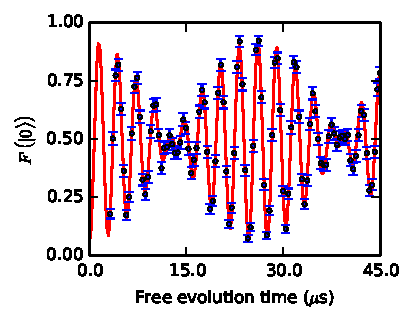
\includegraphics{Img/CarbonRamsey_C1.pdf}
    \caption{Nuclear Ramsey of Carbon 1} \label{fig:CR_C1}
    \end{subfigure}
    \begin{subfigure}[t]{0.49\textwidth}\centering
        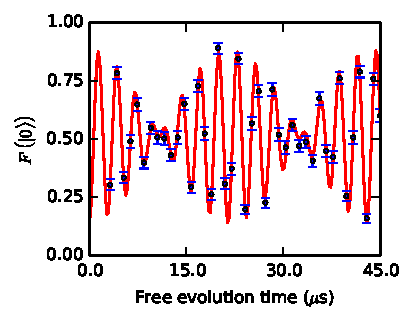
\includegraphics{Img/CarbonRamsey_C4.pdf}
        \caption{Nuclear Ramsey of Carbon 4}
        \label{fig:CR_C4}
    \end{subfigure}
    \caption{Nuclear Ramsey experiment wit}
\end{figure}



\section{Controlling weakly coupled carbons trough the electronic spin}
% Section containing theory (Gate circuits) on how to initialize and readout carbons

Explain how carbon control works in theory.
Explain how a conditional and unconditional gate can be performed.
Explain initialization on gate level, refer to appendix for calculations.
Explain Readout.



\section{Carbon Initialization \& Readout}
% TODO_MAR: Discuss naming of sec: Carbon Init&RO and Carbon Tomo
%  Section containing experimental results (Tomographies)
%  Should emphasize difficulty in seperating initialization and RO fidelity, what is not working? Is it working?
Show results that demonstrate carbon control.



